\documentclass[12pt,msc,a4paper,oneside]{ucl_thesis}
%\documentclass[12pt,mres,draft,a4paper,oneside]{ucl_thesis}

\usepackage{graphicx}
\usepackage{setspace}
\usepackage{amsmath}
\usepackage{url}

\pdfimageresolution=600
% The setspace package lets you use 1.5-sized or double line spacing.
%\setstretch{1.5}

% Title Settings
\setcounter{secnumdepth}{3}
\setcounter{tocdepth}{3}
\title{Alternative Dispute Resolution Using Blockchain Technologies}
\author{Christoph Sitter 
}
    %Supervisor - Prof. Philip Treleaven \\
    %Supervisor - Prof. Tomasz Mloduchowski
\department{Department of Computer Science}

\begin{document}

\maketitle
\makedeclaration

% 02p    - Abstract
%         - 1 - 1.5 pages
%         - Start saying: This dissertation investigates ..., and why this is important
%         - Design, Implemntation, Tests & Results. Factual, keep it brief, no discussion

\setstretch{1.0}
\begin{abstract}
    This thesis investigates the use of Blockchain based technologies for the field of alternative dispute resolution. It starts by investigating scalability as well as safety guarantees and potential risks involved with blockchains and proposes a framework for automated alternative dispute resolution that enables opposing parties to reach a resolution without the need for a neutral third party. 

    The first part of this work investigates the scalability and safety guarantees provided by blockchains to determine whether the requirements for tamper resistance as well as the potential requirement for transaction confirmation in a timely manner, that litigation sometimes requires, can be fulfilled. The majority of this work then focuses on proposing a blockchain based framework that allows conflicting parties to initiate and resolve a dispute. All interactions are kept in an immutable distributed ledger, the blockchain, for future reference as well as provability of claims and statements made. If no mutually satisfying solution can be found, the interactions and documents used in this process can easily be used as evidence in a formal litigation setting. In addition to providing a framework to facilitate disputes, it investigates finding and optimal resolution via cooperation using game theory as defined by Nash.

    The proposed framework defines all components required to provide an end-to-end system for alternative dispute resolution, designed as individual, stand alone, parts that together form a full system. As in normal litigation processes, the first component proposes a tool for discovery. It defines a way to anchor documents into the blockchain, such that it is possible to prove that evidence provided in the discovery phase was seen as well as signed by all involved parties. This is the equivalent of an escrow without the need for an independent third party. All the agreements are implemented using cryptographic operations, and as these operations require safe keeping of keys, a safe way to manage these is proposed as well. 
    The second component is defined as a state machine that details a generic dispute workflow. It investigates the applicability of smart- as well as dumb contracts to implement the state machine with all it's transitions and proposes a template contract that can be used for disputes that follow the defined process. All the components are implemented as a system prototype and tested on a real-world dispute.

\end{abstract}

\setstretch{1.5}
\begin{acknowledgements}
Acknowledge all the things!
\end{acknowledgements}

\setcounter{tocdepth}{2}

\tableofcontents
\listoffigures
\listoftables


\chapter{Introduction}
\label{sec:introduction}

    %TODO: good blog with overview for into? https://ftalphaville.ft.com/2016/04/29/2160502/decentralised-courts-and-blockchains/

    %The system addresses the three areas of legal disputes, and provides a solution that combines the components into a fully functional system. The individual problems are:
    %\begin{itemize}
        %\item Problem 1 - Discovery: Making documents relevant to the claim available to the other party.
        %\item Problem 2 - Dispute: Defining the damages incurred and proposing accepted resolutions.
        %\item Problem 3 - Resolution: Matching proposed resolutions and finding an optimal outcome for both parties (Nash Equilibrium).
    %\end{itemize}
    %In addition to the individual components, a detailed description about the overall architecture of the system as well as a case study using a real case are discussed in this work.

 


%The Blockchain, initially developed as the underlying technology for creating a truly decentralised currency, has found adoption in a variety of fields. Despite it's popularity, the technology is still in very early stages and this thesis investigates some of the scalability as well as security risks involved with using blockchains. 
    %\paragraph*{Problem 1 - Discovery} The first step in every dispute is discovery. Discovery is a pre-trial procedure in which both involved parties can obtain evidence from the other party. Traditionally this is done via lawyers and in a court of law. In our system both parties provide the evidence themselves and anchor it into the Blockchain as a proof that at some point in time they were in possession of the documents. Different cases have different requirements and the system supports anchoring of documents in plain text as well as encrypted versions which the other party will only be able to read if they are given permission or supply documents themselves. The logic behind how documents are shared, encrypted or plain text, is defined in smart contracts.

    %\paragraph*{Problem 2 - Dispute} After discovery has been completed, both parties either start an alternative dispute resolution like mediation or go to trial. This system eliminates the need of a third party in this process by directly linking the two opposing parties via a communications channel on the Blockchain. This provides a traceable and immutable ledger over the interactions between the parties. If neither party agrees to a solution this can be taken as evidence for a future court case.

    %\paragraph*{Problem 3 - Resolution} The last and probably best studied problem is the actual resolution of the dispute. There are multiple ways to resolve a dispute, binding suggestions by the systems, binding agreement between both parties amongst many others. This work looks to mathematically formulate this problem as well as propose a general framework that supports different strategies based on industry best practices.

    %\paragraph*{System Design and Case study} The system design outlines the concept, the interplay between components as well as the systems architecture. It looks into the required infrastructure, access to third party services like smart contract platforms and analyses the security guarantees as well as the load the system can cope with. Finally this design is used to run a case study of a real dispute and it is shown that real-world problems can be resolved without a third party using this system.



%\section{Dispute}
%backup: Either way there is typically a third, neutral, party involved that decides on the final outcome. This poses a problem as this third party can be seen as biased towards one party and hence not neutral or as not knowledgeable enough in the domain to make an informed and fair decision. 

\chapter{Background and Literature Review}
\label{sec:bg_lit_review}

\section{Background}
\subsection{Software development methodology}
The work for this project was subdivided into three stand-alone components that can be considered milestones in an agile setting. The three phases were anchoring data into the blockchain following the chainpoint standard \cite{chainpoint:vaughan}, a platform that uses smart contracts to allow people to start a dispute and attach evidence to the interactions that will all be held in an immutable ledger on a blockchain to ensure that neither the evidence nor the claims can be tampered with and finally an automated system that takes into account the claims as well as the evidence to suggest an ideal resolution to all involved parties. %TODO: Cite smartsettle or similar
Jira was used as a project management platform, on which the roadmap was outlined as stories and tasks. Team members followed Scrum as defined by the agile manifesto and the work was split into weekly sprints to have a fast feedback loop as the team was not co-located. 

\subsection{Source control}
The Git source control facility hosted on the Atlassian Bitbucket infrastructure was used as the version control tool throughout the development process. The project was hosted as a private repository with all member having access to the code. 

\subsection{Programming languages}
For the prototype Python 3 was chosen as the main programming language because of it's flexibility and vast module ecosystem that makes prototyping very fast. In addition to the core language features, the Python module repository provides a multitude of blockchain libraries that create abstractions over the typically low level native APIs. Because of their popularity, the vast community support and the availability of Python modules Bitcoin, detailed in section \ref{sec:background_bitcoin} and Ethereum, detailed in section \ref{sec:background_ethereum} were chosen. 

\subsection{Public key cryptography}
Public key cryptography, sometimes called asymmetric cryptography, is a system which makes use of two distinct keys, a public and a private key. The public key, $K$, can be widely distributed while the private key, $K^{-1}$ must be kept private, as the names suggest. These systems depend on mathematical properties that both keys can be generated easily, but it's computationally intractable to compute the private key, knowing only the public key and encrypted messages $\{m\}_K$. Additionally it is computationally not feasibly to compute $K^{-1}$ or $m$ knowing $\{m\}_K$. Formally, the public key cryptography interface can be defined as [cite DSS lecture]:
\begin{itemize}
    \item{Encrypt: } $E_p(K, m) \rightarrow \{m\}_K$
    \item{Decrypt: } $D_p(K^{-1}, \{m\}) \rightarrow m$
    \item{Sign: }    $S(K^{-1}, m) \rightarrow \{m\}_{K^{-1}}$
    \item{Verify: }  $V(K^{-1}, \{m\}_{K^{-1}}, m) \rightarrow \{true, false\}$
\end{itemize}

While the most popular variants of public key cryptography are the well known RSA and DSA algorithms, as detailed in \cite{RSA:1978:MOD:359340.359342} and [DSA ref needed], elliptic curve cryptography has become more popular in recent years and is the technology used in Bitcoin as well as Ethereum. The main attractiveness of elliptic curve cryptography is that there is currently no sub-exponential algorithm known to solve the discrete logarithm problem for a properly chosen elliptic curve \cite{EllipticCurveOverview}. 

\subsection{Symmetric key cryptography}
Symmetric key cryptography as opposed to asymmetric cryptography is a family of algorithms that use the same key $K$ for encryption as well as decryption. While there exists the drawback of involved parties having to share the secret securely, symmetric algorithms typically are more efficient than asymmetric ones [citation needed]. Formally, symmetric key cryptography can be defined as:
\begin{itemize}
    \item{Encrypt: } $E_s(K, m) -> c$
    \item{Decrypt: } $D_s(K, c) -> m$
\end{itemize}
Symmetric key algorithms are usually used in stream- or block ciphers for use in secure communication channels like SSL/TLS. In the cryptocurrency domain they don't typically aren't used.

\subsection{Cryptographic hash functions}
Bitcoin, described in section \ref{sec:background_bitcoin} as well as Ethereum, described in section \ref{sec:background_ethereum}, at the time of this writing use cryptographic hash functions, SHA-256 to be precise, for the identification of blocks etc. A cryptographic hash function $H$ is a function that takes a plain text $m$ as input and produces an alphanumeric output of fixed length $y = H(m)$. Ideal hash functions should have the following properties [cite DSS \& https://simple.wikipedia.org/wiki/Cryptographic\_hash\_function]:
\begin{itemize}
    \item{Calculating $H(x)$ is computationally easy}
    \item{$H()$ is preimage resistant: } \\ It is computationally infeasible to find $m$ given $y$ and $H$
    \item{$H()$ is second-preimage resistant: } \\ It is computationally infeasible to find $m' \mid y=H(m')=H(m)$ given $y$
\end{itemize}
Because of these properties, cryptographic hash functions are widely used in blockchains and crypto currencies.

\subsection{Elliptic Curve Cryptography overview} \label{sec:background_elliptic_curve}
Write up the maths and find some good illustrations



\let\Btctransaction T
\let\btctransaction t
\let\Btcinput I
\let\btcinput i
\let\Btcoutput O
\let\btcoutput o

\subsection{Bitcoin} \label{sec:background_bitcoin}
It is hard, if not impossible to understate the impact Bitcoin had on the world. Not only has it entirely re-invented how people view a currency, but also introduced blockchain as a technology, without which none of this work would be possible. Bitcoin was designed as a decentralised currency, without a central authority. The main problem it solves is the so called double spending problem, where in theory, the same bitcoin could be spent multiple times without the payee being aware of it. This is solved by timestamping transactions into an immutable distributed ledger, which is realised as an ongoing chain of hash-based proof-of-work. From a technical standpoint, bitcoin can be viewed as a state transition system, operating on a state $S$ defined as:
\begin{equation}
    S := (\Btcinput, \Btcoutput)
\end{equation}
where $\Btcinput$ is the set of transaction inputs and $\Btcoutput$ is the set of transaction outputs as detailed in the next section.

\subsubsection{Bitcoin transactions}
A Bitcoin transaction, defines a transfer of ownership, by consuming one or more unused outputs (UTXO \cite{bitcoin_wiki:utxo}) of a previous transaction, and generating new outputs that the receipient can then again consume and so forth. From a technical perspective, a transaction can be seen as state a state transfer function $S' := \delta_{tx}(S, \Btcinput_{tx}, \Btcoutput_{tx})$. where $\Btcinput_{tx}$ defines the inputs of a transaction and $\Btcoutput_{tx}$ the outputs of this transaction. The function semantics are defined to be:
\begin{equation}
    \delta_{tx}((\Btcinput, \Btcoutput), \Btcinput_{tx}, \Btcoutput_{tx}) := \begin{cases} 
        (\Btcinput \cup \Btcinput_{tx}, \Btcoutput \cup \Btcoutput_{tx}) & if \Btcinput_{tx} \subseteq \Btcoutput \setminus \Btcinput \\
        (\Btcinput, \Btcoutput) & if \Btcinput_{tx} \not\subseteq \Btcoutput \setminus \Btcinput
    \end{cases}
\end{equation}
This means that only transactions, that reference available outputs are considered valid transactions and are hence added to the state. This is an oversimplification of how transactions work and are executed, and it is worth pointing out that a UTXO can only be consumed if the transaction contains proof that it was issued by the holder of the private key associated with the public key in the output. So called coinbase transactions\footnote{Transactions that generate coins without inputs} are also left out, the curious reader however is encouraged to read the bitcoin developer wiki on transactions \cite{bitcoin_wiki:transactions}.

\subsubsection{Timestamping, proof-of-work and mining}
The main problem bitcoin solves is the so called double-spending problem, where two transactions could be spending the same inputs without the payee noticing. To resolve this, it is imperative that there exists a total ordering of transactions, such that all nodes eventually reach the same state $S$.

The solution bitcoin proposes is the so-called blockchan, an ever growing history of blocks containing transactions. A block can loosely be defined as:
\begin{equation}
    B_t := ((H(B_{t-1}, H(n + T), n), T)
\end{equation}
where $H(B_{t-1})$ is the previous block's hash, $H(n + T)$ is the current block's hash, computed from a random nonce $n$ and the transactions contained in this block $T$. This list of transaction containing blocks defines the order in which transactions have occurred. In case that multiple nodes create blocks simultaneously and create a fork on the chain, one fork will eventually outgrow the other and be accepted as the sole truth.

In this simplistic view, it would be easy for an attacker to create a chain that is longer than the existing chain and hence invalidate existing transactions, this problem is solved with the so-called proof-of-work scheme.

\subsection{Proof of Work} \label{sec:background_bitcoin:proof_of_work}
As defined in the previous section, each block contains $H(n + T)$, a hash of the nonce and transactions contained in the block. Proof of work is simply the operation of finding $H(n + T) < threshold$, which due to the underlying cryptographic properties can only be computed by sequentially incrementing the nonce and trying every possible nonce until a valid hash code is produced. In bitcoin the threshold varies and is re-adjusted every 2016 blocks to have an average time of 10 minutes for a new block to be generated. This essentialy means that the longer the chain grows, the harder it is to re-generate it, and it can only be outgrown by a malicious attacker if they control a majority of the networks CPU power.

Because of this proof-of-work scheme, creating a block costs significant CPU time and hence electricity. To incentivise people to put in the investment as well as time, the creator of a new block is rewarded with some bitcoins\footnote{This is somewhat similar to gold miners digging for gold and is hence called mining.} \cite{bitcoin:satoshi}

\subsubsection{Multiple In- and outputs} \label{sec:background_bitcoin:multiple_in_out}
Because of the way bitcoins are transferred, a person controlling 1 bitcoin, may control this one coin as 5 distinct utxos, each worth .2 bitcoins. In order to pay someone 1 bitcoin, the transaction needs to contain all these outputs to transfer a total of 1 bitcoin. Similarly, if a person controls 1 BTC in one single UTXO and they wish to spend 0.5 BTC, then consuming that input and creating a new output worth .5 BTC results in .5 BTC being spent as transaction fees that go to the person mining the block this transaction is in. This is in most cases not desirable, and in order to regain ownership of the remaining .5 BTC, a second output must be added to the transaction transferring the change back to oneself. The difference in amount between all inputs and outputs is considered the transaction fee and can be set arbitrarily, if it is too low however, miners may refuse to include the transaction in their blocks. \cite{bitcoin:satoshi}


\subsection{Ethereum} \label{sec:background_ethereum}
At the time of writing, Ethereum is the second larges crypto currency in the world. Despite this, ethereum was not designed as a crypto currency, but rather a platform for secure distributed computation based on the principles pioneered by Satoshi Nakamoto. 
\subsubsection{Ethereum Transactions}
\subsubsection{Smart Contracts}

\subsection{Chainpoint} \label{sec:literature_chainpoint}
Chainpoint defines a standard for prooving existence of data using blockchains. The idea was pioneered by M. Aroz \cite{proof_of_existence} and is realised by anchoring a cryptographic digest of the document into the public bitcoin blockchain. Chainpoint expanded upon that and defined open standard on top of the initial proof of existence idea to reduce cost and improve scalability.
Blockchains, by design, have a limited transaction throughput and transactions cost money as well as take time to be confirmed. While fees can be optional, they incentivise miners to accept a transaction and add it into a block. In order to reduce the overhead of anchoring multiple documents, chainpoint define a standard that uses a merkle tree for all documents whose root is then anchored and instead a hash of each document itself. The Chainpoint receipt then contains the merkle root, the merkle proof, the target hash and the id of the transaction used for anchoring.

The chainpoint standard aims to be blockchain agnostic and defines receipts for multiple blockchains, at the time of writing, Bitcoin and Ethereum are the only ones supported. It defines how to construct merkle trees with an even as well as uneven number of leaf nodes as and a JSON-LD\footnote{https://json-ld.org/} schema\footnote{https://w3id.org/chainpoint/v2} for the structure of the receipt. Section \ref{chapter:anchoring_data_into_the_blockchain} details how this standard is used in this work.

\subsection{Alternative Dispute Resolution}
When disputes between two parties arise, for example because the customer is not satisfied with the quality of a purchased product and dealing with the trader directly did not lead to a satisfactory resolution, then quite often it is preferable to involve a neutral third party and start one of the many alternative dispute resolution techniques instead of going to court directly. Some of the advantages of alternative dispute resolution methods are that they are generally a lot cheaper, and don't involve the complications that come with having to go to court. \cite{adr_overview:findlaw}

While there do exist countless variants for ADR, the most popular variants are conciliation or mediation, adjudication and arbitration \cite{using_adr:citizensadvice}. 

\subsubsection{Mediation and conciliation}
Mediation is a popular technique for disputes and usually takes place before arbitration. It includes an impartial intermediary that helps the involved to find a mutually acceptable settlement. The solution is not binding and the effectiveness of mediation hence depends on the willingness of all involved parties to come to a mutually beneficial settlement. 

Conciliation typically happens earlier than mediation and focuses on opening communication channels as well as identifying points of mutual agreement. Mediation on the other hand focuses on finding weaknesses in the involved parties arguments and proposing possible mutually acceptable solutions.

Both methods are completely voluntary and the intermediary does not judge, but helps the parties to find a solution themselves. It can be the case that the mediator or conciliator is not impartial and their view may hence not be independent. \cite{using_adr:citizensadvice}

\subsubsection{Adjudication}
Adjudication is a less formal variant of arbitration where an impartial Adjudicator looks at all the written evidence the parties provide and makes a decision. The adjudicator is usually an expert in the field, his decision however is not binding and the problem can be taken to court if the involved parties do not agree with the decision made. \cite{using_adr:citizensadvice}

\subsubsection{Arbitration}
Arbitration is very similar to litigation in the sense that disputants present their arguments to a neutral third party that then decides on a final and imposable resolution that is enforceable in a court of law. Both parties have to agree upfront that they will abide to the decision made by the intermediary. 
The differences to civil litigation are that the involved parties can choose the third party themselves whereas in the judicial system there is typically very little to no control over who will preside as the judge. Another difference is that arbitration is often chosen as a means to start negotiations before an actual dispute materializes whereas the judicial system usually is preferred afterwards. \cite{adr_overview:findlaw}

Arbitration comes in two variants, private- and judicial arbitration. Private Arbitration, the more popular variant, includes two parties who contractually agree to adhere to the decision made by the arbitrator which usually is a private person chosen by all involved parties upfront. The arbitrators decision is binding. Judicial arbitration is usually court imposed and the decision made by the arbitrator is non-binding, meaning that any party dissatisfied with the decision has the right to formally appeal and take the claim to court. Typically this has to be done within a certain time limit decided upon by the court and if this is exceeded the decision becomes binding just as with private arbitration.

\subsubsection{Remarks}
ADR techniques have gained popularity in recent years and there are countless variants of the outlined methods. In all ADR techniques facilitating negotiations between the involved parties plays an important role, but it is important to note that they are not the right choice for all legal disputes. One major factor is that parties involved in ADR usually waive their right to object to evidence that might be inadmissible in a court of law - one example of this is hearsay.

\section{Literature Review and Related Work}
This section investigates existing services and research that is relevant to the area of blockchain based alternative dispute resolution. 

\section{Blockchain based notary-like services}
In legal disputes, it is imperative, that guarantees about the existence of documents can be made as well as the ability to proof interactions between parties. In ADR this would typically be a neutral third party, which has, amongst others, notary-like roles. 

While the range of services provided by notaries is by far not restricted to the ones mentioned here, for the purpose of this work only two are required. Witnessing and certifying the validity of signatures on documents as well as certifying the authenticity of the document itself. \cite{notary:does_blockchain_notary_work}

The blockchain can satisfy both of these requirements, using arbitrary data embedded into transactions as detailed in chapter \ref{chapter:anchoring_data_into_the_blockchain}, it can be proven that a document existed at a given point in time, and the person that put the document there can proof that it was them putting it there using public/private key cryptography. 

There do exist a variety of online services attempting to replace notaries using a public blockchain, some popular ones are the following, as taken from \cite{notary:does_blockchain_notary_work}:

\begin{itemize}
    \item{\textbf{Bitproof:}} Created by 18 year old Louison Dumont. The process requires users to record a video of themselves though as part of the process.
    \item{\textbf{BlockSign:}} Must be a pdf but is a free service.
    \item{\textbf{ProveBit:}} Links to a github code repository.
    \item{\textbf{Stampd:}} Simple and effective. Costs 9 cents.
    \item{\textbf{Stampery:}} Not an online service. More enterprise and consultancy focused. Great Medium post though.
    \item{\textbf{Proof of Existence:}} Same technical process under the hood. Different (more accurate?) angle.
    \item{\textbf{Tierion:}} Online blockchain based data store, as part of this work an open-source version of this service was implemented, detailed in chapter \ref{chapter:anchoring_data_into_the_blockchain}
\end{itemize}

While these services come close to providing some of the services of a notary, one major shortcoming is that it is not possible to proof that it was a certain person putting the document there. Stampery propose to use NameCoin\footnote{\url{https://namecoin.org}} to assign an identity to a document, this however has not been implemented or tested yet, and there is no guarantee that a fraudulent attacker couldn't register a fake name to impersonate someone else \cite{notary:does_blockchain_notary_work} \cite{notary:stampery_medium}.


\chapter{Safety guarantees of and attacks on the blockchain}

\section{Ellyptic curve cryptography}
\section{Coping with Moore's law}
\section{Double spending problem and confirmations}
\section{The 51\% attack}
\section{Forks and implications on security}
\section{Mining and the tragedy of the commons}
\section{Transaction throughput}


\chapter{Disclosure - Anchoring data into the blockchain} \label{chapter:anchoring_data_into_the_blockchain}
English law [citation needed\footnote{http://newsroom.howardkennedy.com/disclosure-of-documents-in-international-arbitration-a-solution-for-globalised-trade/}] does not formally define the process of disclosure for ADR, as opposed to a well defined set of rules for formal litigation. The parties involved in the dispute typically agree on a form of ADR as well as the rules they wish to follow. This chapter formally defines disclosure as a state machine and proposes a generic framework for multiple parties to disclose and inspect documents based on cryptographic proofs and guarantees. In order to minimise the dependencies on any particular blockchain, the following definitions all assume no specific underlying blockchain and propose a micro transaction protocol that can be run on top of an existing blockchain without the need for an account with funds to pay transaction fees.


\section{Formalising Disclosure} \label{sec:formalising_disclosure}
There are many different ways to perform disclosure, and depending on the type of ADR as well as the domain of the dispute, financial, civil etc, the process can vary. In civil litigation full disclosure is usually recommended, while in financial disputes the involved parties may choose not to disclose confidential information to the other party, but only to the intermediary. In this chapter we formally define how disclosure can be performed using blockchain technologies without a third party invovement based on the ADR workflow defined in figure \ref{fig:adr_workflow}.


Disclosure is merely the claim that a document exist, where the disclosing party has an obligation to produce the document should the other party request inspection of it. This is loosely based on UK civil procedure rules as defined in \cite{justice_gov:civil_procedure_rules}. To perform disclosure without the involvment of a third party, a disclosed document must provide three guarantees:
\begin{enumerate}
    \item{\textbf{Proof of existence:}} It must be possible for any of the involved parties to proof that a document existed at a certain time in the past. \label{itm:disclosure_document_objectives_existence}
    
    \item{\textbf{Proof of disclosure:}} It must be possible for any involved party to proof that a document was disclosed by another involved party. \label{itm:disclosure_document_objectives_disclosure}

    \item{\textbf{Secrecy against evesdropper:}} Secrecy of the document exchanges must be guaranteed, that means that while eavesdroppers may be able to intercept that two parties are communicating, the identity as well as details of the interaction must remain secure. \label{itm:disclosure_document_objectives_evesdrop}
   
    \item{\textbf{Secrecy of confidential information amongs parties:}} It must be possible to obfuscate confidential information such that the counterparty will only know of it's existence and information that is willingly provided. It must also be possible to later on produce the confidential document in a verifiable manner. \label{itm:disclosure_document_objectives_confidential}

    \item{\textbf{Proof of identity of involved parties:}} It is desirable for each party to have the ability to proof the identity of the party that has disclosed documents for the purpose of possible follow up formal litigation processes. This is investigated in chapter \ref{chapter:key_management}. [TODO: Figure out if we want that and if so how] \label{itm:disclosure_document_objectives_identification}
\end{enumerate}
In order to meet the above mentioned objectives while remaining blockchain agnostic, a micro transaction framework is devised that is based on the definitions provided in the following sections:

\subsection{Definition of Document} \label{sec:definition_of_document}
A Document is defined as a composite of the document and cryptographic proofs to meet the objectives set out in the previous section. Formally a document is defined as the quintuple:
\begin{equation}
    d := (K_o, H(c), t, S(K_o^{-1}, (K_o, t, H(c))), c) 
    \label{eq:disclosure_document}
\end{equation}

This quintuple is composed of the public key of the disclosing party $K_o$, a cryptographic hash $H(c)$ of the possibly encrypted document $c$, a plaintext description or title $t$, the signature $S$ of the triple $(K_o, t, H(c))$ using the private key of the disclosing party $K_o^{-1}$ and the ciphertext $c$ representing the encrypted document. In this work, $c := E_s(K_d, m)$ is generated using a symmetric key cryptographic function, using a dedicated key per document $K_d$, there do exist more sophisticated mechanisms like multi party computation to securely share encrypted data with no one party knowing the full key, but this is out of scope and considered future work.

\subsection{Definition of Receipt} \label{sec:definition_of_receipt}
Once a document $d$ is generated, a cryptographic hash $H(d)$ is anchored into the blockchain using the system described in section \ref{sec:disclosure_anchor_data}. The anchoring system generates a Chainpoint receipt to proof the existence of a document later on. For the purpose of this work, an ADR receipt is defined as the quadruple:
\begin{equation}
    \psi := (r_d, d, K_i, S(K_i^{-1}, (r_d, d, K_i)))
    \label{eq:disclosure_receipt}
\end{equation}
where $r_d$ is the Chainpoint receipt generated by the anchoring system, $K_i$ the public key of the party the document was disclosed to and $S(K_i^{-1}, (r_d, d, K_i))$ a cryptographic signature proving that the party holding the private key $K_i^{-1}$ associated with the public key $K_i$ has recieved the document.


\subsection{Definition of the disclosure protocol}
The disclosure protocol can loosely be defined as a state machine with state 
\begin{equation}
    S := \{\Psi, R, D | \psi \in \Psi, r \in R, d \in D\}
    \label{eq:disclosure_state_machine}
\end{equation}
and state transfer functions $\delta_{add}$, $\delta_{anchor}$, $\delta_{ack}$ modify the state of the system $S' := \delta_x(S) \forall x \in \{add, anchor, ack\}$ and are formally defined as:
\begin{equation}
    \{\Psi, R, D \cup d\} := \delta_{add}(\{\Psi, R, D\}, d)
    \label{eq:disclosure_delta_add}
\end{equation}
\begin{equation}
    \{\Psi, R \cup r, D\} := \delta_{anchor}(\{\Psi, R, D\}, d)
    \label{eq:disclosure_delta_anchor}
\end{equation}
\begin{equation}
    \{\Psi \cup \psi, R \setminus r, D \setminus d\} := \delta_{ack}(\{\Psi, R, D\}, r)
    \label{eq:disclosure_delta_ack}
\end{equation}
Informally, $\delta_{add}$ can be seen as preparing the document for anchoring, $\delta_{anchor}$ as producing a proof of existence for the document ad $\delta_{ack}$ as the counter party acknowledging the receipt of the document. After the protocol has completed, both parties are in possession of the receipt $\psi$. This receipt can be used to meet the objectives set in section \ref{sec:formalising_disclosure}, and how this is achieved is described in the following section.

\subsection{Applicability of the protocol to defined objectives}
This section describes how an adr receipt $\psi$ can be used to meed the objectives set for the system, in particular:
\begin{enumerate}
    \item{\textbf{Proof of existence:}} The Chainpoint receipt $r$ contains information about the block that $H(d)$ and can hence be used to proof that the document existed before the said block was generated.
    \item{\textbf{Proof of disclosure:}} The ADR receipt $\psi$ contains a signature of the receiving party, proving that they have received the document $d$ included in the receipt. The receiving party has the ability to proof that the receipt is for the document provided.
    \item{\textbf{Secrecy against evesdropper:}} Assuming the communication channel between the opposing parties is not secure, then encrypting each document with it's unique key provides secrecy against evesdroppers. 
    \item{\textbf{Secrecy of confidential information amongs parties:}} As all documents are encrypted with a secret key, it is easily possible to send a document to the other party while withholding the key, effectively proving that the document exists but not disclosing it's contents.
    \item{\textbf{Proof of identity of involved parties:}} The outlined protocol provides no guarantees about the identity of parties behind the public keys, this problem is addressed in chapter \ref{chapter:key_management}.
\end{enumerate}

\begin{figure}
    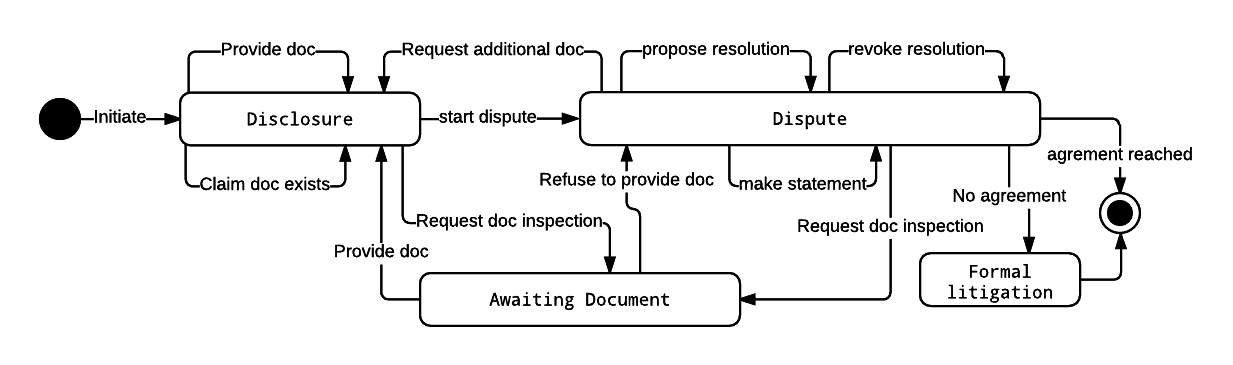
\includegraphics[width=1.0\textwidth,trim={.5cm 15cm 7.5cm 1cm},clip]{./figures/adr_workflow.png}
    \caption{ADR Workflow}
    \label{fig:adr_workflow}
\end{figure}

\section{Anchoring data into the Blockchain} \label{sec:disclosure_anchor_data}
In the first phase of this project, an open source version of Tierion\footnote{\url{https://tierion.com/}} was implemented that is then used as the framework to produce proof of existence and is available on \url{TODO: figure out where}. The system exposes a REST API equivalent to the one defined by Tierion and aims to be a drop in replacement.

\subsection{Library Design}
The 

\subsection{Bitcoin}
\subsection{Ethereum}
\section{Tierion and the Chainpoint standard}
\section{Library and API design}

\chapter{Key Management} \label{chapter:key_management}
problems with mediation: -- no mediator is smart enough, are they really neutral etc etc

\chapter{Dispute - definition and smart contract proposal}

\section{Dispute as a state machine}
\section{Smart contract template for dispute}


\chapter{Resolution}
\section{Game theoretic view of dispute resolution}
\section{Definition of actions and resolution}
\section{System design}

\chapter{Experiment - Emulating a real dispute on the prototype}
\section{Discovery}
\section{Dispute}
\section{Resolution}

\bibliographystyle{unsrt}
\bibliography{bibliography}
\end{document}
